% Options for packages loaded elsewhere
\PassOptionsToPackage{unicode}{hyperref}
\PassOptionsToPackage{hyphens}{url}
%
\documentclass[
]{article}
\usepackage{lmodern}
\usepackage{amssymb,amsmath}
\usepackage{ifxetex,ifluatex}
\ifnum 0\ifxetex 1\fi\ifluatex 1\fi=0 % if pdftex
  \usepackage[T1]{fontenc}
  \usepackage[utf8]{inputenc}
  \usepackage{textcomp} % provide euro and other symbols
\else % if luatex or xetex
  \usepackage{unicode-math}
  \defaultfontfeatures{Scale=MatchLowercase}
  \defaultfontfeatures[\rmfamily]{Ligatures=TeX,Scale=1}
\fi
% Use upquote if available, for straight quotes in verbatim environments
\IfFileExists{upquote.sty}{\usepackage{upquote}}{}
\IfFileExists{microtype.sty}{% use microtype if available
  \usepackage[]{microtype}
  \UseMicrotypeSet[protrusion]{basicmath} % disable protrusion for tt fonts
}{}
\makeatletter
\@ifundefined{KOMAClassName}{% if non-KOMA class
  \IfFileExists{parskip.sty}{%
    \usepackage{parskip}
  }{% else
    \setlength{\parindent}{0pt}
    \setlength{\parskip}{6pt plus 2pt minus 1pt}}
}{% if KOMA class
  \KOMAoptions{parskip=half}}
\makeatother
\usepackage{xcolor}
\IfFileExists{xurl.sty}{\usepackage{xurl}}{} % add URL line breaks if available
\IfFileExists{bookmark.sty}{\usepackage{bookmark}}{\usepackage{hyperref}}
\hypersetup{
  pdftitle={Project 1},
  pdfauthor={Mai Le},
  hidelinks,
  pdfcreator={LaTeX via pandoc}}
\urlstyle{same} % disable monospaced font for URLs
\usepackage[margin=1in]{geometry}
\usepackage{color}
\usepackage{fancyvrb}
\newcommand{\VerbBar}{|}
\newcommand{\VERB}{\Verb[commandchars=\\\{\}]}
\DefineVerbatimEnvironment{Highlighting}{Verbatim}{commandchars=\\\{\}}
% Add ',fontsize=\small' for more characters per line
\usepackage{framed}
\definecolor{shadecolor}{RGB}{248,248,248}
\newenvironment{Shaded}{\begin{snugshade}}{\end{snugshade}}
\newcommand{\AlertTok}[1]{\textcolor[rgb]{0.94,0.16,0.16}{#1}}
\newcommand{\AnnotationTok}[1]{\textcolor[rgb]{0.56,0.35,0.01}{\textbf{\textit{#1}}}}
\newcommand{\AttributeTok}[1]{\textcolor[rgb]{0.77,0.63,0.00}{#1}}
\newcommand{\BaseNTok}[1]{\textcolor[rgb]{0.00,0.00,0.81}{#1}}
\newcommand{\BuiltInTok}[1]{#1}
\newcommand{\CharTok}[1]{\textcolor[rgb]{0.31,0.60,0.02}{#1}}
\newcommand{\CommentTok}[1]{\textcolor[rgb]{0.56,0.35,0.01}{\textit{#1}}}
\newcommand{\CommentVarTok}[1]{\textcolor[rgb]{0.56,0.35,0.01}{\textbf{\textit{#1}}}}
\newcommand{\ConstantTok}[1]{\textcolor[rgb]{0.00,0.00,0.00}{#1}}
\newcommand{\ControlFlowTok}[1]{\textcolor[rgb]{0.13,0.29,0.53}{\textbf{#1}}}
\newcommand{\DataTypeTok}[1]{\textcolor[rgb]{0.13,0.29,0.53}{#1}}
\newcommand{\DecValTok}[1]{\textcolor[rgb]{0.00,0.00,0.81}{#1}}
\newcommand{\DocumentationTok}[1]{\textcolor[rgb]{0.56,0.35,0.01}{\textbf{\textit{#1}}}}
\newcommand{\ErrorTok}[1]{\textcolor[rgb]{0.64,0.00,0.00}{\textbf{#1}}}
\newcommand{\ExtensionTok}[1]{#1}
\newcommand{\FloatTok}[1]{\textcolor[rgb]{0.00,0.00,0.81}{#1}}
\newcommand{\FunctionTok}[1]{\textcolor[rgb]{0.00,0.00,0.00}{#1}}
\newcommand{\ImportTok}[1]{#1}
\newcommand{\InformationTok}[1]{\textcolor[rgb]{0.56,0.35,0.01}{\textbf{\textit{#1}}}}
\newcommand{\KeywordTok}[1]{\textcolor[rgb]{0.13,0.29,0.53}{\textbf{#1}}}
\newcommand{\NormalTok}[1]{#1}
\newcommand{\OperatorTok}[1]{\textcolor[rgb]{0.81,0.36,0.00}{\textbf{#1}}}
\newcommand{\OtherTok}[1]{\textcolor[rgb]{0.56,0.35,0.01}{#1}}
\newcommand{\PreprocessorTok}[1]{\textcolor[rgb]{0.56,0.35,0.01}{\textit{#1}}}
\newcommand{\RegionMarkerTok}[1]{#1}
\newcommand{\SpecialCharTok}[1]{\textcolor[rgb]{0.00,0.00,0.00}{#1}}
\newcommand{\SpecialStringTok}[1]{\textcolor[rgb]{0.31,0.60,0.02}{#1}}
\newcommand{\StringTok}[1]{\textcolor[rgb]{0.31,0.60,0.02}{#1}}
\newcommand{\VariableTok}[1]{\textcolor[rgb]{0.00,0.00,0.00}{#1}}
\newcommand{\VerbatimStringTok}[1]{\textcolor[rgb]{0.31,0.60,0.02}{#1}}
\newcommand{\WarningTok}[1]{\textcolor[rgb]{0.56,0.35,0.01}{\textbf{\textit{#1}}}}
\usepackage{graphicx,grffile}
\makeatletter
\def\maxwidth{\ifdim\Gin@nat@width>\linewidth\linewidth\else\Gin@nat@width\fi}
\def\maxheight{\ifdim\Gin@nat@height>\textheight\textheight\else\Gin@nat@height\fi}
\makeatother
% Scale images if necessary, so that they will not overflow the page
% margins by default, and it is still possible to overwrite the defaults
% using explicit options in \includegraphics[width, height, ...]{}
\setkeys{Gin}{width=\maxwidth,height=\maxheight,keepaspectratio}
% Set default figure placement to htbp
\makeatletter
\def\fps@figure{htbp}
\makeatother
\setlength{\emergencystretch}{3em} % prevent overfull lines
\providecommand{\tightlist}{%
  \setlength{\itemsep}{0pt}\setlength{\parskip}{0pt}}
\setcounter{secnumdepth}{-\maxdimen} % remove section numbering

\title{Project 1}
\author{Mai Le}
\date{3/3/2020}

\begin{document}
\maketitle

\begin{Shaded}
\begin{Highlighting}[]
\CommentTok{###Data sets}
\KeywordTok{library}\NormalTok{(tidyverse)}
\NormalTok{USArrests<-}\KeywordTok{read.csv}\NormalTok{(}\StringTok{"USArrests.csv"}\NormalTok{)}
\NormalTok{StatesEdu<-}\KeywordTok{read.csv}\NormalTok{(}\StringTok{"StatesEdu.csv"}\NormalTok{)}
\KeywordTok{glimpse}\NormalTok{(USArrests)}
\end{Highlighting}
\end{Shaded}

\begin{verbatim}
## Observations: 50
## Variables: 5
## $ State    <fct> AL, AK, AZ, AR, CA, CO , CN, DE, FL, GA, HI, ID, IL, IN, I...
## $ Murder   <dbl> 13.2, 10.0, 8.1, 8.8, 9.0, 7.9, 3.3, 5.9, 15.4, 17.4, 5.3,...
## $ Assault  <int> 236, 263, 294, 190, 276, 204, 110, 238, 335, 211, 46, 120,...
## $ UrbanPop <int> 58, 48, 80, 50, 91, 78, 77, 72, 80, 60, 83, 54, 83, 65, 57...
## $ Rape     <dbl> 21.2, 44.5, 31.0, 19.5, 40.6, 38.7, 11.1, 15.8, 31.9, 25.8...
\end{verbatim}

\begin{Shaded}
\begin{Highlighting}[]
\KeywordTok{glimpse}\NormalTok{(StatesEdu)}
\end{Highlighting}
\end{Shaded}

\begin{verbatim}
## Observations: 51
## Variables: 8
## $ State   <fct> AL, AK, AZ, AR, CA, CO, CN, DE, DC, FL, GA, HI, ID, IL, IN,...
## $ region  <fct> ESC, PAC, MTN, WSC, PAC, MTN, NE, SA, SA, SA, SA, PAC, MTN,...
## $ pop     <int> 4041, 550, 3665, 2351, 29760, 3294, 3287, 666, 607, 12938, ...
## $ SATV    <int> 470, 438, 445, 470, 419, 456, 430, 433, 409, 418, 401, 404,...
## $ SATM    <int> 514, 476, 497, 511, 484, 513, 471, 470, 441, 466, 443, 481,...
## $ percent <int> 8, 42, 25, 6, 45, 28, 74, 58, 68, 44, 57, 52, 17, 16, 54, 5...
## $ dollars <dbl> 3.648, 7.887, 4.231, 3.334, 4.826, 4.809, 7.914, 6.016, 8.2...
## $ pay     <int> 27, 43, 30, 23, 39, 31, 43, 35, 39, 30, 29, 32, 25, 34, 32,...
\end{verbatim}

My first dataset StatesEdu contains related statistics on the education
in US States and Washington DC. It has 5 variables including State,
Murder (murder arrests per 100000), Assault (assault arrests per
100000), UrbanPop (percent urban population), and Rape (rape arrests per
100000). My second dataset USArrests contains information on violent
crime rate in different States. It has 8 variables including State,
region (of the US), pop (population in 1000s), SATV (average score of
graduating high school students in state on the verbal component of
Scholastic Aptidtude Test), SATM (average score of graduating high
school student in the state on the math component of Scholastic Aptitude
Test), percent (of graduating high school students in the state who took
the SAT exam), dollars (state spending on public education in 1000s
dollars per student), and pay (average teacher's salary in the state in
1000s dollars).

I found these two from the vincentarelbundock website of archive of R
datasets. They were interesting to me because there have been much talk
about education relating to the safety of our communities in the
political debate that's currently happening. I think there will be an
inverse correlation between the dollars in the StatesEdu and at least
one of the arrests variable in the USArrests, if not all of them.

\begin{Shaded}
\begin{Highlighting}[]
\CommentTok{###Joining}
\CommentTok{#observation CO in USArrests contains a space whereas CO in StatesEdu doesn't}
\CommentTok{#to get rid of the space}
\NormalTok{USArrests<-USArrests}\OperatorTok\KeywordTok{mutate}\NormalTok{(}\DataTypeTok{State=}\KeywordTok{str_trim}\NormalTok{(State,}\StringTok{"right"}\NormalTok{)) }
\NormalTok{bothdata<-}\KeywordTok{inner_join}\NormalTok{(USArrests, StatesEdu, }\DataTypeTok{by=}\StringTok{"State"}\NormalTok{)}
\NormalTok{bothdata}
\end{Highlighting}
\end{Shaded}

\begin{verbatim}
##   State Murder Assault UrbanPop Rape region   pop SATV SATM percent dollars pay
## 1    AL   13.2     236       58 21.2    ESC  4041  470  514       8   3.648  27
## 2    AK   10.0     263       48 44.5    PAC   550  438  476      42   7.887  43
## 3    AZ    8.1     294       80 31.0    MTN  3665  445  497      25   4.231  30
## 4    AR    8.8     190       50 19.5    WSC  2351  470  511       6   3.334  23
## 5    CA    9.0     276       91 40.6    PAC 29760  419  484      45   4.826  39
## 6    CO    7.9     204       78 38.7    MTN  3294  456  513      28   4.809  31
## 7    CN    3.3     110       77 11.1     NE  3287  430  471      74   7.914  43
## 8    DE    5.9     238       72 15.8     SA   666  433  470      58   6.016  35
##  [ reached 'max' / getOption("max.print") -- omitted 42 rows ]
\end{verbatim}

\begin{Shaded}
\begin{Highlighting}[]
\KeywordTok{anti_join}\NormalTok{(USArrests,StatesEdu)}
\end{Highlighting}
\end{Shaded}

\begin{verbatim}
## [1] State    Murder   Assault  UrbanPop Rape    
## <0 rows> (or 0-length row.names)
\end{verbatim}

\begin{Shaded}
\begin{Highlighting}[]
\KeywordTok{anti_join}\NormalTok{(StatesEdu,USArrests)}
\end{Highlighting}
\end{Shaded}

\begin{verbatim}
##   State region pop SATV SATM percent dollars pay
## 1    DC     SA 607  409  441      68    8.21  39
\end{verbatim}

I used inner\_join to combine my two dataset together by keeping only
the rows that have a match on the ID variable of State. I used this one
because I wanted to drop any row in either datset that doesn't have a
match, which was the observation of DC in the StatesEdu dateset. I found
this by using anti\_join to give me the rows in one dataset that have no
match in the other dataset and vice versa. One resulting potential
problem its information won't be incoporated to help find any possible
correlation between different variables later on.

\begin{Shaded}
\begin{Highlighting}[]
\CommentTok{###Wrangling}
\KeywordTok{summary}\NormalTok{(bothdata}\OperatorTok{$}\NormalTok{pay)}
\end{Highlighting}
\end{Shaded}

\begin{verbatim}
##    Min. 1st Qu.  Median    Mean 3rd Qu.    Max. 
##   22.00   27.25   30.00   30.78   33.00   43.00
\end{verbatim}

\begin{Shaded}
\begin{Highlighting}[]
\NormalTok{bothdata<-bothdata}\OperatorTok\KeywordTok{group_by}\NormalTok{(pay)}\OperatorTok
\StringTok{  }\KeywordTok{mutate}\NormalTok{(}\DataTypeTok{pay_cat =} \KeywordTok{case_when}\NormalTok{(pay}\OperatorTok{>}\DecValTok{36}\OperatorTok{~}\StringTok{"high"}\NormalTok{,}\DecValTok{29}\OperatorTok{<=}\NormalTok{pay }\OperatorTok{&}
\StringTok{  }\NormalTok{pay}\OperatorTok{<=}\DecValTok{36} \OperatorTok{~}\StringTok{"med"}\NormalTok{,pay}\OperatorTok{<}\DecValTok{29}\OperatorTok{~}\StringTok{"low"}\NormalTok{))}

\NormalTok{bothdata<-bothdata}\OperatorTok\StringTok{ }\KeywordTok{mutate}\NormalTok{(}\DataTypeTok{percent_cat=}\KeywordTok{factor}\NormalTok{(}\KeywordTok{ntile}\NormalTok{(percent,}\DecValTok{2}\NormalTok{),}
  \DataTypeTok{levels=}\DecValTok{1}\OperatorTok{:}\DecValTok{2}\NormalTok{,}\DataTypeTok{labels=}\KeywordTok{c}\NormalTok{(}\StringTok{"lower"}\NormalTok{,}\StringTok{"higher"}\NormalTok{)))}

\NormalTok{bothdata}\OperatorTok\KeywordTok{filter}\NormalTok{(region}\OperatorTok{==}\StringTok{"SA"}\NormalTok{)}\OperatorTok\KeywordTok{select}\NormalTok{(State,pay_cat,Assault)}\OperatorTok
\StringTok{  }\KeywordTok{arrange}\NormalTok{(}\KeywordTok{desc}\NormalTok{(Assault))}
\end{Highlighting}
\end{Shaded}

\begin{verbatim}
## # A tibble: 8 x 4
## # Groups:   pay [7]
##     pay State pay_cat Assault
##   <int> <chr> <chr>     <int>
## 1    29 NC    med         337
## 2    30 FL    med         335
## 3    38 MD    high        300
## 4    28 SC    low         279
## 5    35 DE    med         238
## 6    29 GA    med         211
## 7    32 VA    med         156
## 8    26 WV    low          81
\end{verbatim}

\begin{Shaded}
\begin{Highlighting}[]
\CommentTok{#finding summary statistics for each numeric variable overall}
\NormalTok{bothdata}\OperatorTok\KeywordTok{mutate}\NormalTok{(}\DataTypeTok{sdSATM=}\KeywordTok{sd}\NormalTok{(SATM,}\DataTypeTok{na.rm=}\NormalTok{T))}
\end{Highlighting}
\end{Shaded}

\begin{verbatim}
## # A tibble: 50 x 15
## # Groups:   pay [20]
##    State Murder Assault UrbanPop  Rape region   pop  SATV  SATM percent dollars
##    <chr>  <dbl>   <int>    <int> <dbl> <fct>  <int> <int> <int>   <int>   <dbl>
##  1 AL      13.2     236       58  21.2 ESC     4041   470   514       8    3.65
##  2 AK      10       263       48  44.5 PAC      550   438   476      42    7.89
##  3 AZ       8.1     294       80  31   MTN     3665   445   497      25    4.23
##  4 AR       8.8     190       50  19.5 WSC     2351   470   511       6    3.33
##  5 CA       9       276       91  40.6 PAC    29760   419   484      45    4.83
##  6 CO       7.9     204       78  38.7 MTN     3294   456   513      28    4.81
##  7 CN       3.3     110       77  11.1 NE      3287   430   471      74    7.91
##  8 DE       5.9     238       72  15.8 SA       666   433   470      58    6.02
##  9 FL      15.4     335       80  31.9 SA     12938   418   466      44    5.15
## 10 GA      17.4     211       60  25.8 SA      6478   401   443      57    4.86
## # ... with 40 more rows, and 4 more variables: pay <int>, pay_cat <chr>,
## #   percent_cat <fct>, sdSATM <dbl>
\end{verbatim}

\begin{Shaded}
\begin{Highlighting}[]
\CommentTok{#finding summary statistics for numeric variable after grouping}
\NormalTok{bothdata}\OperatorTok\KeywordTok{group_by}\NormalTok{(percent_cat)}\OperatorTok\KeywordTok{summarize}\NormalTok{(}\KeywordTok{max}\NormalTok{(pop))}
\end{Highlighting}
\end{Shaded}

\begin{verbatim}
## # A tibble: 2 x 2
##   percent_cat `max(pop)`
##   <fct>            <int>
## 1 lower            29760
## 2 higher           16987
\end{verbatim}

\begin{Shaded}
\begin{Highlighting}[]
\NormalTok{bothdata}\OperatorTok\KeywordTok{group_by}\NormalTok{(percent_cat)}\OperatorTok\KeywordTok{summarize}\NormalTok{(}\KeywordTok{median}\NormalTok{(dollars))}
\end{Highlighting}
\end{Shaded}

\begin{verbatim}
## # A tibble: 2 x 2
##   percent_cat `median(dollars)`
##   <fct>                   <dbl>
## 1 lower                    4.84
## 2 higher                   5.05
\end{verbatim}

\begin{Shaded}
\begin{Highlighting}[]
\NormalTok{bothdata}\OperatorTok\KeywordTok{group_by}\NormalTok{(percent_cat)}\OperatorTok\KeywordTok{summarize_at}\NormalTok{(}\KeywordTok{c}\NormalTok{(}\StringTok{"UrbanPop"}\NormalTok{,}\StringTok{"pop"}\NormalTok{,}\StringTok{"pay"}\NormalTok{), var)}
\end{Highlighting}
\end{Shaded}

\begin{verbatim}
## # A tibble: 2 x 4
##   percent_cat UrbanPop       pop   pay
##   <fct>          <dbl>     <dbl> <dbl>
## 1 lower           195. 37425353.  29.5
## 2 higher          240. 18720384.  24.8
\end{verbatim}

\begin{Shaded}
\begin{Highlighting}[]
\NormalTok{bothdata}\OperatorTok\KeywordTok{group_by}\NormalTok{(region)}\OperatorTok\KeywordTok{summarize}\NormalTok{(}\KeywordTok{mean}\NormalTok{(pay))}
\end{Highlighting}
\end{Shaded}

\begin{verbatim}
## # A tibble: 9 x 2
##   region `mean(pay)`
##   <fct>        <dbl>
## 1 ENC           33.8
## 2 ESC           27  
## 3 MA            38.7
## 4 MTN           28  
## 5 NE            34.3
## 6 PAC           35.8
## 7 SA            30.9
## 8 WNC           27  
## 9 WSC           25.2
\end{verbatim}

\begin{Shaded}
\begin{Highlighting}[]
\NormalTok{bothdata}\OperatorTok\StringTok{ }\KeywordTok{group_by}\NormalTok{(region)}\OperatorTok\KeywordTok{summarize}\NormalTok{(}\KeywordTok{cor}\NormalTok{(dollars, SATM))}
\end{Highlighting}
\end{Shaded}

\begin{verbatim}
## # A tibble: 9 x 2
##   region `cor(dollars, SATM)`
##   <fct>                 <dbl>
## 1 ENC                   0.526
## 2 ESC                   0.241
## 3 MA                    0.999
## 4 MTN                  -0.110
## 5 NE                   -0.293
## 6 PAC                  -0.876
## 7 SA                    0.661
## 8 WNC                  -0.161
## 9 WSC                  -0.613
\end{verbatim}

\begin{Shaded}
\begin{Highlighting}[]
\NormalTok{bothdata}\OperatorTok\KeywordTok{group_by}\NormalTok{(region)}\OperatorTok\KeywordTok{summarize_at}\NormalTok{(}\KeywordTok{c}\NormalTok{(}\StringTok{"Assault"}\NormalTok{,}\StringTok{"Murder"}\NormalTok{,}\StringTok{"Rape"}\NormalTok{), IQR)}
\end{Highlighting}
\end{Shaded}

\begin{verbatim}
## # A tibble: 9 x 4
##   region Assault Murder  Rape
##   <fct>    <dbl>  <dbl> <dbl>
## 1 ENC      136     3.2   3   
## 2 ESC       73.5   1.60  5.72
## 3 MA        74     2.4   5.6 
## 4 MTN      140.    3.62 17.6 
## 5 NE        75.8   1.25  2.57
## 6 PAC      118     4.1  14.4 
## 7 SA       112.    6.8  10.3 
## 8 WNC       44.5   2.7   5.20
## 9 WSC       32.8   5.12  3.15
\end{verbatim}

\begin{Shaded}
\begin{Highlighting}[]
\NormalTok{bothdata}\OperatorTok\KeywordTok{group_by}\NormalTok{(pay_cat)}\OperatorTok\KeywordTok{summarize}\NormalTok{(}\KeywordTok{cor}\NormalTok{(UrbanPop,percent))}
\end{Highlighting}
\end{Shaded}

\begin{verbatim}
## # A tibble: 3 x 2
##   pay_cat `cor(UrbanPop, percent)`
##   <chr>                      <dbl>
## 1 high                      0.336 
## 2 low                      -0.0192
## 3 med                      -0.147
\end{verbatim}

\begin{Shaded}
\begin{Highlighting}[]
\CommentTok{#one statistic from grouping two categorical variables }
\NormalTok{bothdata}\OperatorTok\KeywordTok{group_by}\NormalTok{(region,pay_cat)}\OperatorTok\KeywordTok{summarize_at}\NormalTok{(}\StringTok{"SATV"}\NormalTok{,}
\NormalTok{  min)}\OperatorTok\KeywordTok{pivot_wider}\NormalTok{(}\DataTypeTok{names_from=}\NormalTok{pay_cat,}\DataTypeTok{values_from=}\NormalTok{SATV)}
\end{Highlighting}
\end{Shaded}

\begin{verbatim}
## # A tibble: 9 x 4
## # Groups:   region [9]
##   region  high   med   low
##   <fct>  <int> <int> <int>
## 1 ENC      454   408    NA
## 2 ESC       NA   473   470
## 3 MA       412   420    NA
## 4 MTN       NA   434   464
## 5 NE       422   427   423
## 6 PAC      419   404    NA
## 7 SA       430   401   397
## 8 WNC       NA   477   473
## 9 WSC       NA    NA   413
\end{verbatim}

The standard deviations for average score of graduating high school
student in the state on the math copmonent of Scholastic Aptitude Test
overall range from 2.828427 to 52.648837. The maximum population is
higher in the lower category of percent of graduating high school
students in the state who took the SAT while its median percent state
spending on public education is lower. The variance of poulation and
average teacher's salary in the state is higher for lower category of
percent of graduating high school students while the opposite is seen
for urban population. The mean average teacher's salary ranges not too
far apart between the different US regions. 5 regions have negative
correlation between dollars (state spending on public education) and
average score of graduating high school students in the state on the
math component while 4 other regions have positive correlation. The
interquartile ranges of murder and rape arrests are much lower than that
of the assault arrest. Average teacher's salary that falls within the
high category is the only one with a positive correlation between urban
population and percent of graduating high school students in the state
who took the SAT. Meanwhile, the low and medium categories both have
negative correlation. After grouping the data by US region and tidying
it, the medium category of the average of teacher's salary has the
highest average score of graduating high school students in the state on
the verbal component while the low category had the lowest value. The
high category seems to have the smallest range of scores while the low
category has the biggest.

\begin{Shaded}
\begin{Highlighting}[]
\CommentTok{###Visualizing (correlation heatmap of numeric variables)}
\NormalTok{bothdata}\OperatorTok\KeywordTok{select_if}\NormalTok{(is.numeric)}\OperatorTok\NormalTok{cor}\OperatorTok\NormalTok{as.data.frame}\OperatorTok
\StringTok{  }\NormalTok{rownames_to_column}\OperatorTok\KeywordTok{pivot_longer}\NormalTok{(}\OperatorTok{-}\DecValTok{1}\NormalTok{)}\OperatorTok\KeywordTok{ggplot}\NormalTok{(}\KeywordTok{aes}\NormalTok{(rowname,name,}\DataTypeTok{fill=}\NormalTok{value))}\OperatorTok{+}
\StringTok{  }\KeywordTok{geom_tile}\NormalTok{()}\OperatorTok{+}\KeywordTok{geom_text}\NormalTok{(}\KeywordTok{aes}\NormalTok{(}\DataTypeTok{label=}\KeywordTok{round}\NormalTok{(value,}\DecValTok{2}\NormalTok{)))}\OperatorTok{+}\KeywordTok{xlab}\NormalTok{(}\StringTok{""}\NormalTok{)}\OperatorTok{+}\KeywordTok{ylab}\NormalTok{(}\StringTok{""}\NormalTok{)}\OperatorTok{+}
\StringTok{  }\KeywordTok{theme}\NormalTok{(}\DataTypeTok{axis.text.x =} \KeywordTok{element_text}\NormalTok{(}\DataTypeTok{angle =} \DecValTok{90}\NormalTok{, }\DataTypeTok{hjust =} \DecValTok{1}\NormalTok{))}\OperatorTok{+}
\StringTok{  }\KeywordTok{scale_fill_gradient2}\NormalTok{(}\DataTypeTok{low=}\StringTok{"red"}\NormalTok{,}\DataTypeTok{high=}\StringTok{"blue"}\NormalTok{)}
\end{Highlighting}
\end{Shaded}

\begin{center}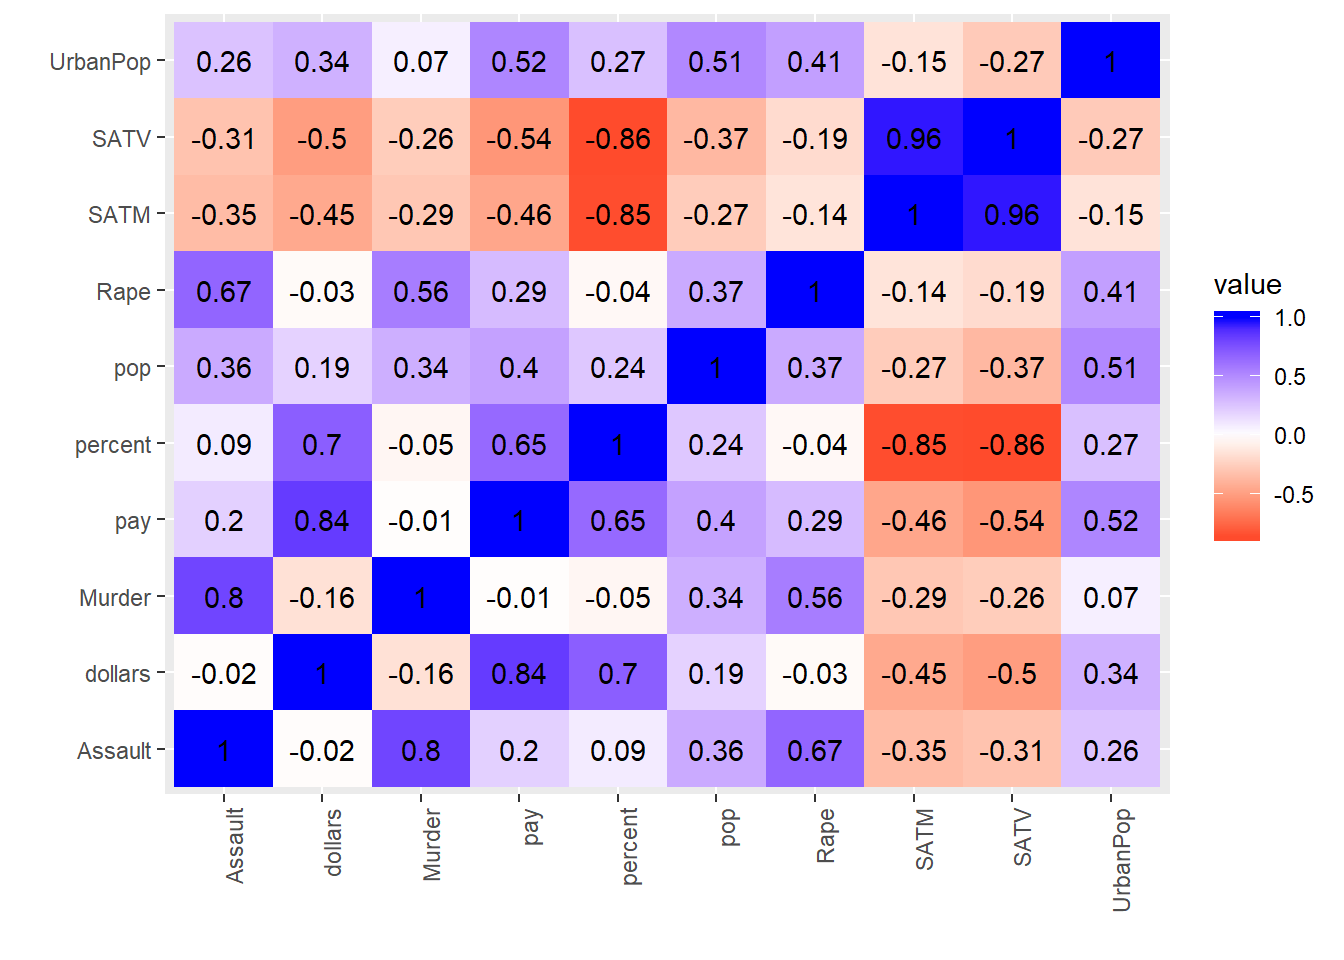
\includegraphics{project1_files/figure-latex/unnamed-chunk-5-1} \end{center}

The average scores of graduating high school students in the state on
the math and verbal component have negative correlation with all the
other variables, except when it's with each other. Urban population has
a postive correlation with all the other, except when it's with the two
variables mentioned earlier. Population also has a positive correaltion
with all the other variables. Besides the two SAT scores the strong
positive correlation is between average teacher's salary and state's
spending on public education (dollars). Meanwhile, the strongest
negative correlations were between the percent of graduating high school
students who took the SAT and the average score of graduating high
school students in the state on the math and verbal component.

\begin{Shaded}
\begin{Highlighting}[]
\CommentTok{###Visualizing (ggplot 1)}
\KeywordTok{ggplot}\NormalTok{(bothdata, }\KeywordTok{aes}\NormalTok{(}\DataTypeTok{x=}\NormalTok{region, }\DataTypeTok{y=}\NormalTok{Murder, }\DataTypeTok{fill=}\NormalTok{percent_cat))}\OperatorTok{+}
\StringTok{  }\KeywordTok{scale_fill_hue}\NormalTok{(}\DataTypeTok{l=}\DecValTok{40}\NormalTok{)}\OperatorTok{+}\KeywordTok{geom_bar}\NormalTok{(}\DataTypeTok{stat=}\StringTok{"summary"}\NormalTok{, }\DataTypeTok{fun.y=}\StringTok{"mean"}\NormalTok{)}\OperatorTok{+}
\StringTok{  }\KeywordTok{ggtitle}\NormalTok{(}\StringTok{"Bar Chart of Murder Arrests vs Percent vs US Region"}\NormalTok{) }\OperatorTok{+}
\StringTok{  }\KeywordTok{scale_y_continuous}\NormalTok{(}\DataTypeTok{breaks=}\KeywordTok{seq}\NormalTok{(}\DecValTok{0}\NormalTok{,}\DecValTok{35}\NormalTok{,}\DecValTok{5}\NormalTok{))}\OperatorTok{+}\KeywordTok{xlab}\NormalTok{(}\StringTok{"Regions of US"}\NormalTok{)}\OperatorTok{+}\StringTok{ }
\StringTok{  }\KeywordTok{ylab}\NormalTok{(}\StringTok{"Murder Arrests per 1000,000"}\NormalTok{) }\OperatorTok{+}\KeywordTok{theme}\NormalTok{(}\DataTypeTok{axis.text.x=}\KeywordTok{element_text}\NormalTok{(}\DataTypeTok{angle=}\DecValTok{90}\NormalTok{,}\DataTypeTok{hjust=}\DecValTok{1}\NormalTok{))}
\end{Highlighting}
\end{Shaded}

\begin{center}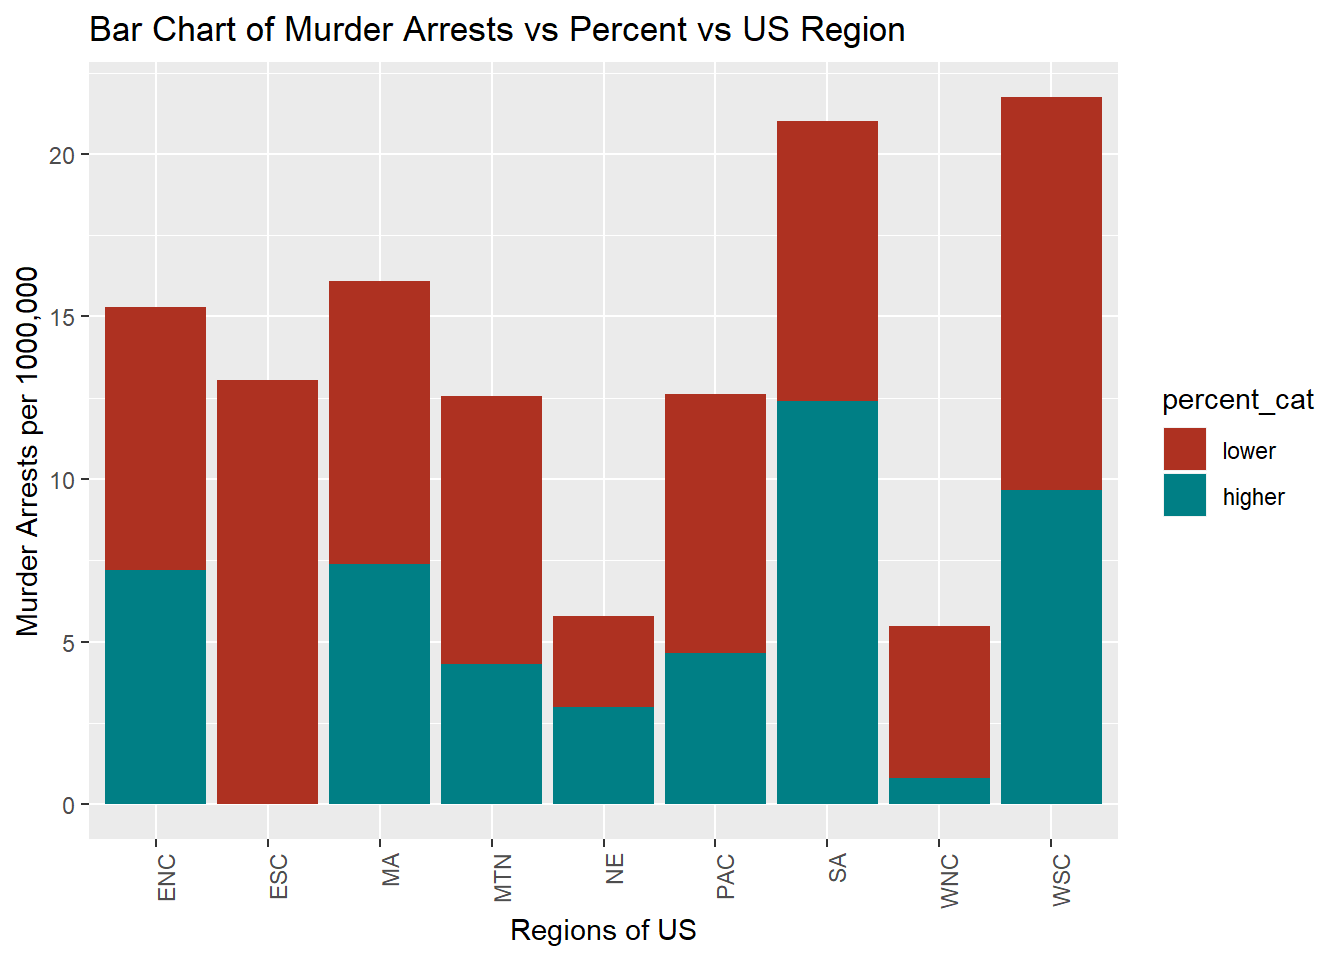
\includegraphics{project1_files/figure-latex/unnamed-chunk-6-1} \end{center}

From the bar chart, there seems to be higher murder arrests per 1000,000
if the percent of graduating high school students in the state who took
the SAT exam falls under the lower category that compared to the higher
one in the same US region. One exception is that of NE region where the
higher category of percent of graduating high school students in the
state who took the SAT exam seems to have a slightly higher murder
arrests than that of the lower percent category. The two regions with
the highest murder arrests are WSC and SA while the lowest were NE and
WNC.

\begin{Shaded}
\begin{Highlighting}[]
\CommentTok{###Visualizing (ggplot 2)}
\KeywordTok{ggplot}\NormalTok{(bothdata, }\KeywordTok{aes}\NormalTok{(Assault, Rape, }\DataTypeTok{color=}\NormalTok{dollars))}\OperatorTok{+}\KeywordTok{geom_point}\NormalTok{()}\OperatorTok{+}
\StringTok{  }\KeywordTok{ggtitle}\NormalTok{(}\StringTok{"Scatterplot of Assault Arrest, Rape Arrests, }
\StringTok{  and State's Spending on Public Education"}\NormalTok{)}\OperatorTok{+}
\StringTok{  }\KeywordTok{scale_color_gradient}\NormalTok{(}\DataTypeTok{low=}\StringTok{"yellow"}\NormalTok{, }\DataTypeTok{high=}\StringTok{"red"}\NormalTok{)}\OperatorTok{+}
\StringTok{  }\KeywordTok{xlab}\NormalTok{(}\StringTok{"Assault Arrests per 100,000"}\NormalTok{)}\OperatorTok{+}\KeywordTok{ylab}\NormalTok{(}\StringTok{"Rape Arrests per 100,000"}\NormalTok{)}\OperatorTok{+}\KeywordTok{theme_dark}\NormalTok{()}
\end{Highlighting}
\end{Shaded}

\begin{center}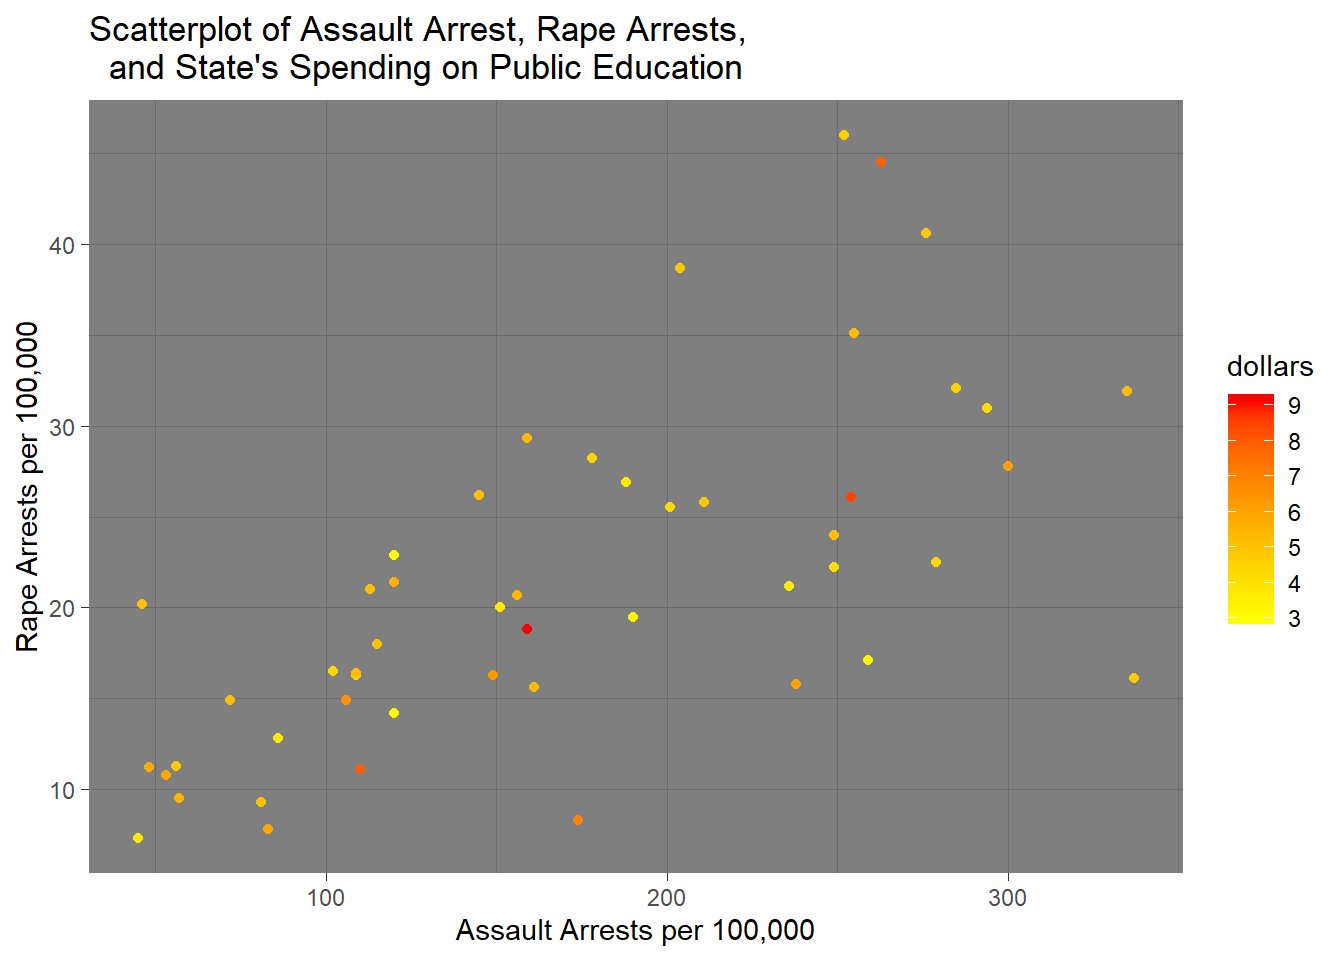
\includegraphics{project1_files/figure-latex/unnamed-chunk-7-1} \end{center}

From the plot above, there seems to be a general positive correlation
between the Assault Arrests and the Rape Arrests per 100,000. If a
regression line was generated, we can see as Assault Arrests increases,
the Rape Arrests seem to increase as well with a few outliers. On the
other hand, there doesn't seem to be any prominent relationship between
dollar vairable (state spending on public education in 1000s dollars per
student) with either of the two variables. This can be concluded from
the color gradient being distributed everywhere on the plot, with no
visible trend either to the x-axis or the y-axis.

\begin{Shaded}
\begin{Highlighting}[]
\CommentTok{###Dimentionality Reduction}
\KeywordTok{library}\NormalTok{(ggplot2)}
\KeywordTok{library}\NormalTok{(cluster)}

\CommentTok{#choosing number of clusters}
\NormalTok{variables<-bothdata}\OperatorTok\KeywordTok{select}\NormalTok{(Rape,pay,percent,pop)}
\NormalTok{sil_width<-}\KeywordTok{vector}\NormalTok{()}
\ControlFlowTok{for}\NormalTok{(i }\ControlFlowTok{in} \DecValTok{2}\OperatorTok{:}\DecValTok{10}\NormalTok{)\{}
\NormalTok{  pam_fit <-}\StringTok{ }\KeywordTok{pam}\NormalTok{(variables, }\DataTypeTok{k=}\NormalTok{i)}
\NormalTok{  sil_width[i] <-}\StringTok{ }\NormalTok{pam_fit}\OperatorTok{$}\NormalTok{silinfo}\OperatorTok{$}\NormalTok{avg.width}
\NormalTok{\}}
\KeywordTok{ggplot}\NormalTok{()}\OperatorTok{+}\KeywordTok{geom_line}\NormalTok{(}\KeywordTok{aes}\NormalTok{(}\DataTypeTok{x=}\DecValTok{1}\OperatorTok{:}\DecValTok{10}\NormalTok{,}\DataTypeTok{y=}\NormalTok{sil_width))}\OperatorTok{+}\KeywordTok{scale_x_continuous}\NormalTok{(}\DataTypeTok{name=}\StringTok{"k"}\NormalTok{,}\DataTypeTok{breaks=}\DecValTok{1}\OperatorTok{:}\DecValTok{10}\NormalTok{)}
\end{Highlighting}
\end{Shaded}

\begin{center}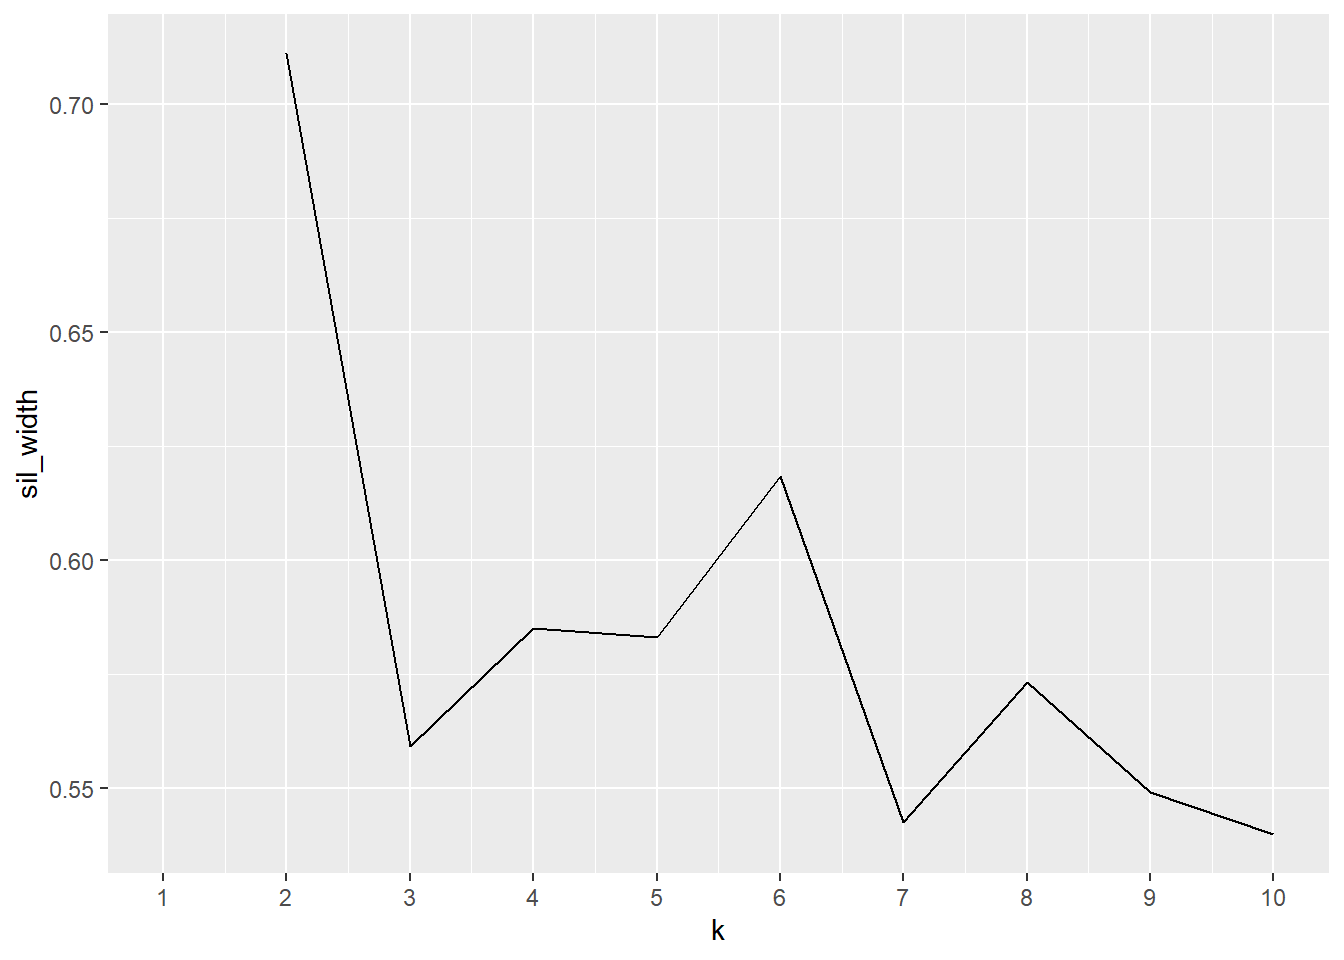
\includegraphics{project1_files/figure-latex/unnamed-chunk-8-1} \end{center}

\begin{Shaded}
\begin{Highlighting}[]
\CommentTok{#interpreting Average Silhouette Width}
\NormalTok{pam1<-}\StringTok{ }\NormalTok{variables}\OperatorTok\KeywordTok{pam}\NormalTok{(}\DecValTok{2}\NormalTok{)}
\KeywordTok{plot}\NormalTok{(pam1, }\DataTypeTok{which=}\DecValTok{2}\NormalTok{) }
\end{Highlighting}
\end{Shaded}

\begin{center}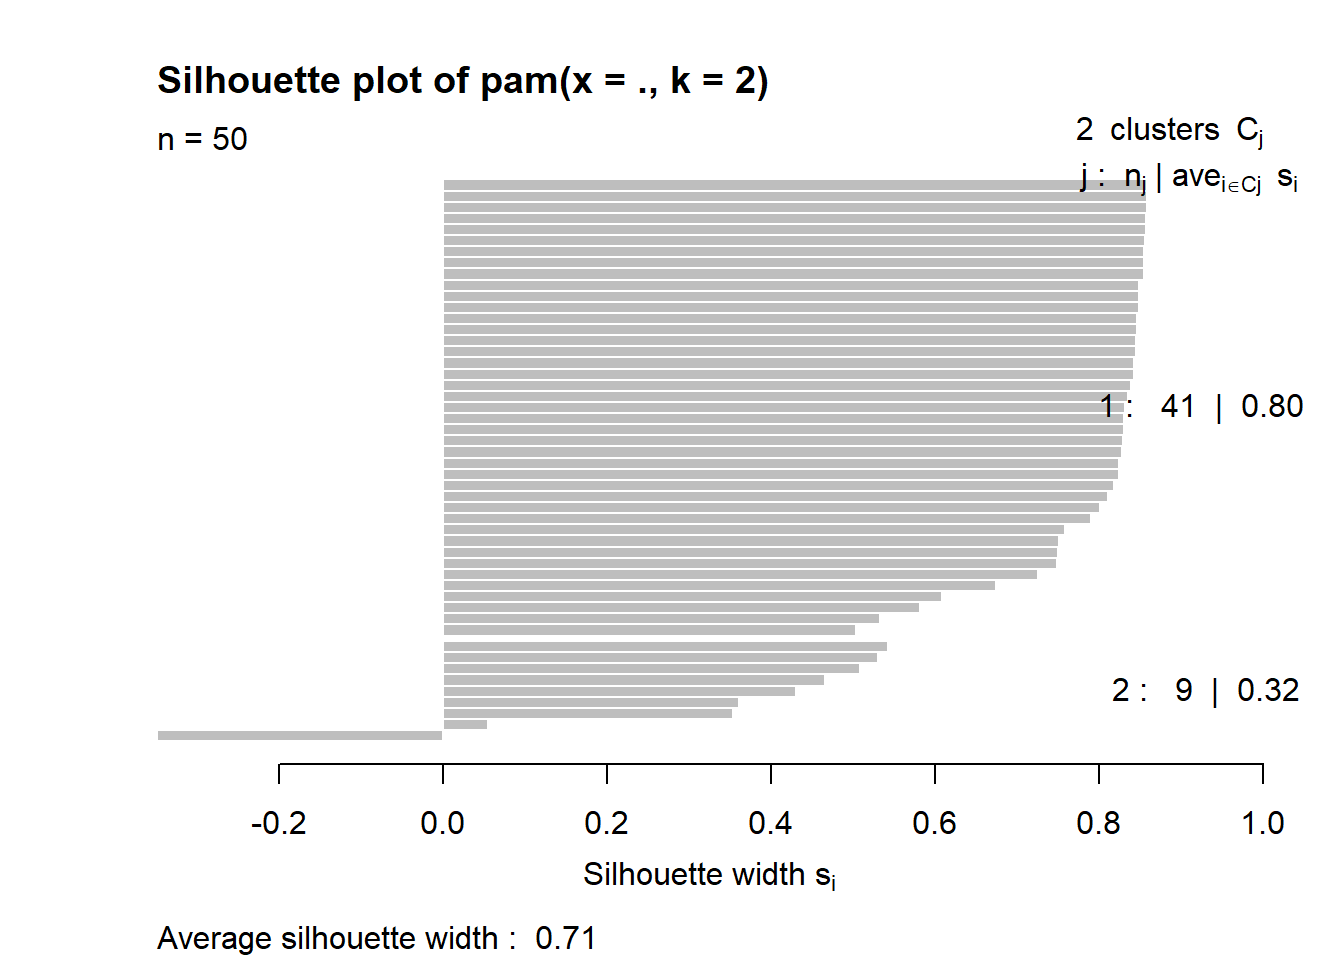
\includegraphics{project1_files/figure-latex/unnamed-chunk-8-2} \end{center}

\begin{Shaded}
\begin{Highlighting}[]
\KeywordTok{library}\NormalTok{(GGally)}

\CommentTok{#visualize pairwise combinations}
\NormalTok{pamclust<-variables}\OperatorTok\NormalTok{ungroup}\OperatorTok\KeywordTok{mutate}\NormalTok{(}\DataTypeTok{cluster=}\KeywordTok{as.factor}\NormalTok{(pam1}\OperatorTok{$}\NormalTok{clustering))}
\NormalTok{pamclust}\OperatorTok\StringTok{ }\KeywordTok{ggpairs}\NormalTok{(}\DataTypeTok{columns =} \KeywordTok{c}\NormalTok{(}\DecValTok{1}\NormalTok{,}\DecValTok{2}\NormalTok{,}\DecValTok{3}\NormalTok{,}\DecValTok{4}\NormalTok{), }\KeywordTok{aes}\NormalTok{(}\DataTypeTok{color=}\NormalTok{cluster))}
\end{Highlighting}
\end{Shaded}

\begin{center}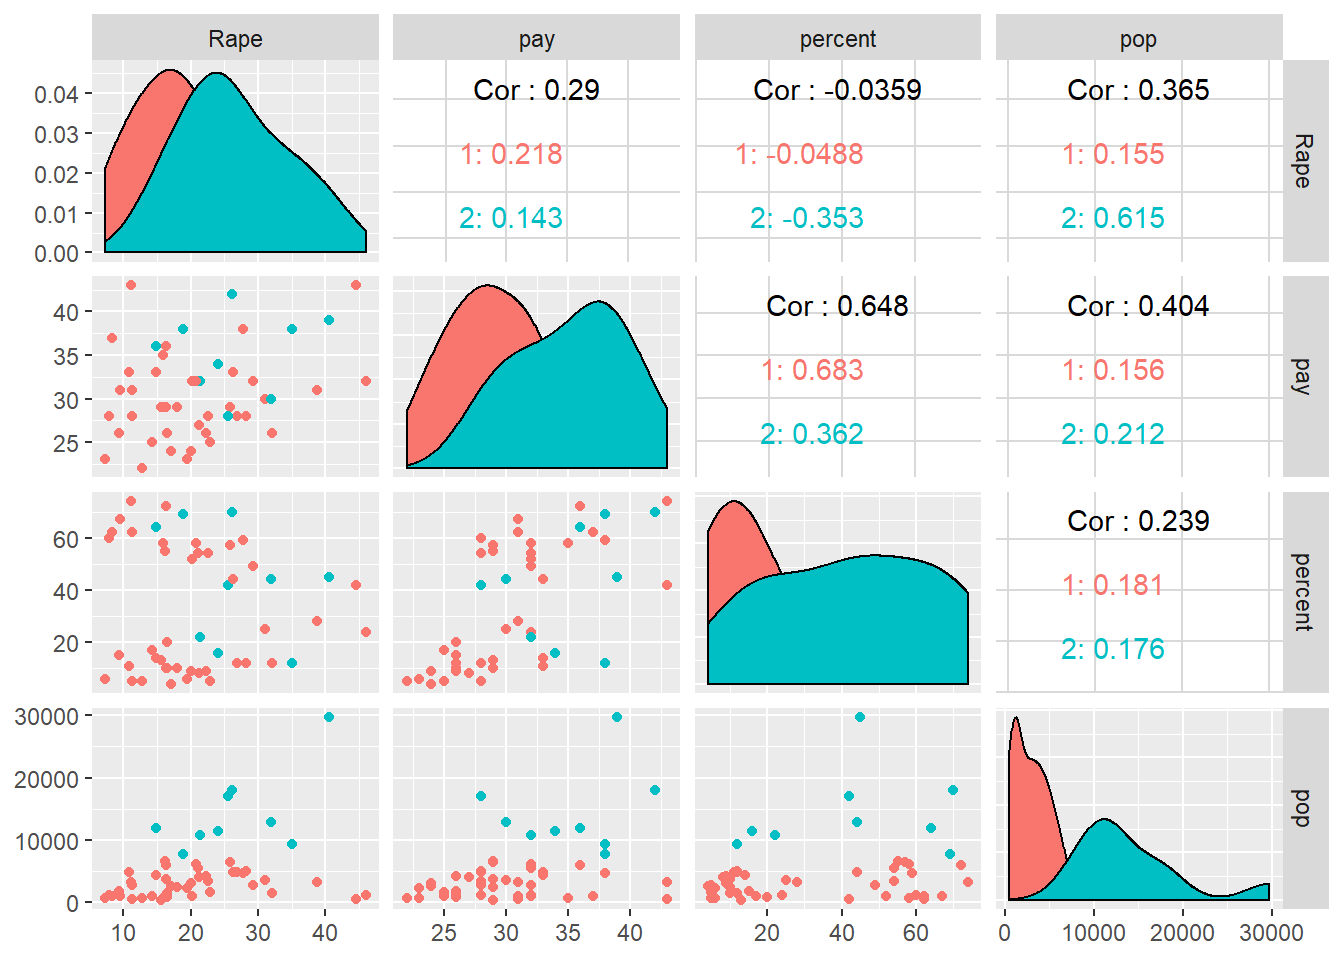
\includegraphics{project1_files/figure-latex/unnamed-chunk-8-3} \end{center}

I created a smaller dataset of just Rape, pay, percent, and pop
variables to analyze since I think they might have interesting results
to look at. Then, I chose a cluster of 2 by running mean silhouette
width, and the highest peak in the plot was 2 for k. The average
silhouette width was 0.71, indicating that a strong structure has been
found. I then created a visualization of all the possible pair of
combination to compare between those 4 variables. All pairs have weak
positive correlation except percent (of high school stdents in the state
who took the SAT exam) with Rape Arrests, which had a weak very negative
correlation. Percent (of high school stdents in the state who took the
SAT exam) and pay (average teacher's salary) have a higher positive
correlation than the other combination pairs.

\end{document}
